\documentclass[11pt]{article}
\usepackage[margin=1in]{geometry}
\usepackage{amsmath,array,booktabs,graphicx,hyperref,caption,threeparttable,longtable}
\newcolumntype{L}[1]{>{\raggedright\arraybackslash}p{#1}}
\usepackage[round]{natbib}
\usepackage[section]{placeins}
\hypersetup{colorlinks=true,linkcolor=blue,citecolor=blue,urlcolor=blue}
\captionsetup{font=small,labelfont=bf}
\newcommand{\Vcoin}{\$103}
\newcommand{\VcoinLo}{\$100}
\newcommand{\VcoinHi}{\$106}
\newcommand{\VcoinPct}{1.03\%}
\newcommand{\VcoinStd}{\$148}
\newcommand{\VcoinStdLo}{\$143}
\newcommand{\VcoinStdHi}{\$152}
\newcommand{\VcoinStdPct}{1.48\%}
\newcommand{\Vconv}{\$33}
\newcommand{\Vskill}{\$285}
\newcommand{\VskillLo}{\$281}
\newcommand{\VskillHi}{\$290}
\newcommand{\VskillConv}{\$149}
\newcommand{\VskillStd}{\$405}
\newcommand{\SizingGain}{\$70}
\newcommand{\SkillGain}{\$182}
\newcommand{\Dval}{$-$\$112}
\newcommand{\DvalLo}{$-$\$117}
\newcommand{\DvalHi}{$-$\$107}
\newcommand{\Ppass}{24.7\%}
\newcommand{\Ppaid}{15.5\%}
\newcommand{\PpassExact}{0.247}
\newcommand{\PpaidExact}{0.155}
\newcommand{\VperFunded}{\$418}
\newcommand{\ShareFundedPaid}{63\%}
\newcommand{\PaidMedian}{\$537}
\newcommand{\PaidPninetyfive}{\$1,604}
\newcommand{\EVpromo}{\$63}
\newcommand{\EVlist}{$-$\$44}
\newcommand{\BEsharpeList}{$-$0.05}
\newcommand{\SkillEqSizing}{0.04}
\newcommand{\SkillEqPromo}{0.14}
\newcommand{\CoinSharpe}{$-$0.21}
\newcommand{\CoinCost}{0.0069}
\newcommand{\CoinSd}{0.51}
\newcommand{\HitThree}{52.1\%}
\newcommand{\HitOne}{55.0\%}
\newcommand{\HitTwo}{59.1\%}
\newcommand{\HitZero}{50.9\%}
\newcommand{\TradeDays}{4,879}
\newcommand{\Lam}{1.74}
\newcommand{\Vmedian}{1.21\%}
\newcommand{\CapStd}{2.1\%}
\newcommand{\Pref}{6,952}
\newcommand{\VcoinOnePct}{\$33}
\newcommand{\PpassOnePct}{9\%}
\newcommand{\VcoinHalfRf}{\$56}
\newcommand{\VskillOne}{\$886}
\newcommand{\VskillTwo}{\$2,307}
\newcommand{\Npaths}{50,000}
\newcommand{\MdeMedian}{0.77}
\newcommand{\RefutedThree}{5}
\newcommand{\RefutedFive}{12}
\newcommand{\DenialPromo}{61\%}

\newcommand{\DclockTwelve}{\$3.5 (1.9 to 5.2)}
\newcommand{\DnoneSixty}{$-$\$245}
\newcommand{\VcoinClock}{\$76}
\newcommand{\VcoinNoCutoff}{\$105}
\newcommand{\ClockCostCoin}{28\%}
\newcommand{\ClockCostThree}{35\%}
\newcommand{\ClockCostOne}{43\%}
\newcommand{\ForfeitTwelve}{96\%}
\newcommand{\ForfeitTwentyFour}{79\%}
\newcommand{\ForfeitThirtySix}{62\%}
\newcommand{\ForfeitSixty}{42\%}
\newcommand{\StillEvalTwelve}{70\%}
\newcommand{\StillEvalThirtySix}{20\%}
\newcommand{\CautiousOne}{\$689}
\newcommand{\CautiousMultiple}{6.5}
\newcommand{\BookLo}{0.58\%}
\newcommand{\BookHi}{1.31\%}
\newcommand{\VNas}{\$131}
\newcommand{\VEur}{\$95}
\newcommand{\VJpy}{\$58}
\newcommand{\VbestCoin}{\$120}
\newcommand{\GainBestCoin}{16\%}
\newcommand{\PpassBest}{28.5\%}
\newcommand{\PpaidBest}{18.2\%}
\newcommand{\VbestCoinPct}{1.20\%}
\newcommand{\GainBestThree}{7\%}
\newcommand{\GainBestOne}{11\%}
\newcommand{\GainBestOneStd}{43\%}
\newcommand{\GainTimingOneStd}{22\%}
\newcommand{\ModelRatio}{1.06}
\newcommand{\EvalRiskCoin}{4.2\%}
\newcommand{\EvalRiskThree}{1.6\%}
\newcommand{\EvalRiskOne}{1.7\%}
\newcommand{\SpanMedian}{10}
\newcommand{\SpanNinety}{32}
\newcommand{\PerFeeMin}{\$0.49}
\newcommand{\PerFeeMax}{\$1.60}
\newcommand{\PerFeeSwing}{\$0.70}
\newcommand{\PerFeeProTen}{\$1.42}
\newcommand{\PerFeeProTenLarge}{\$2.44}
\newcommand{\VProTen}{\$109}
\newcommand{\EVProTen}{\$32}
\newcommand{\DiffProSwing}{\$6}
\newcommand{\VProTenBi}{\$122}
\newcommand{\VDirect}{\$91}
\newcommand{\PpaidDirect}{13\%}
\newcommand{\VOneTen}{\$46}
\newcommand{\DiffOnePro}{\$63}
\newcommand{\VProTenSkill}{\$303}
\newcommand{\VOneSixSkill}{\$71}
\newcommand{\VAoneLate}{\$155}
\newcommand{\VAoneLateLo}{\$10}
\newcommand{\VAoneLateHi}{\$320}
\newcommand{\VAoneEarly}{\$468}
\newcommand{\IdealAoneLate}{\$397}
\newcommand{\VRthreeLate}{\$17}
\newcommand{\IdealRthreeLate}{\$292}
\newcommand{\SharpeRthreeLate}{0.32}
\newcommand{\VWthreeLate}{\$80}
\newcommand{\CoinLate}{\$96}
\newcommand{\VslipFive}{\$88}
\newcommand{\VslipTen}{\$75}
\newcommand{\VslipTwentyFive}{\$49}
\newcommand{\BonusCoin}{\$0.85}
\newcommand{\BonusOne}{\$10.74}

\makeatletter\newcommand{\tabin}[1]{\@@input #1.tex }\makeatother
\newcommand{\RepoNote}{\url{https://github.com/coderback/prop-challenge-pricing}}

\title{Fair on Paper:\\ What a Prop-Firm Challenge Is Worth, and Who Pays for It}
\author{Timothy Oluwatobi Ojebiyi\thanks{Independent researcher, United Kingdom. Email:
\href{mailto:tobiojebiyi@gmail.com}{tobiojebiyi@gmail.com}. Code, the dated analysis plans, rule sources and result
tables: \RepoNote. Disclosure: I hold a free demonstration account on the firm's trading server, which I used to
measure its spreads. I have never bought one of its evaluations or received a payment from it, and I have no
commercial relationship with any firm in this industry. Nothing in this paper is investment advice or a
recommendation to buy any product. I used Anthropic's Claude to assist with code and drafting; I verified all design
choices, results and conclusions and take full responsibility for them. All errors are mine.}}
\date{Draft, October 2026}

\begin{document}
\maketitle

\begin{abstract}
\noindent
Retail ``prop firms'' sell evaluation contracts: a fee buys a simulated account, and a buyer who reaches a profit
target without breaching loss limits is paid a share of later simulated profits. I price the full published
contract of a named UK firm on twenty years of intraday index prices at measured broker costs, with every
hypothesis fixed and time-stamped before its run. Three results stand out. First, the written rules are close to a
fair bet for a disciplined buyer with no skill: expected payouts are about \VcoinPct{} of the account on the base
contract, between \BookLo{} and \BookHi{} across four instruments, against list fees of 0.3\% to 1.5\%. Second, the
price list does not follow contract value. Across the firm's nine plans the same buyer gets back between
\PerFeeMin{} and \PerFeeMax{} per dollar of fee, and one plan sells the same targets and limits as another at half
the price. Third, the contract pays steeply for skill, but for a kind of skill a pre-registered search did not
find: an idealised Sharpe ratio of 0.3 is worth \Vskill{} per \$10,000 account, while the one strategy ensemble
that survived to untouched data is worth \VRthreeLate{}. The rules are therefore not where the seller's margin
comes from. It comes from how buyers size and trade, from an edge they lack and cannot verify, and from the firm's
published discretion over the conduct that extracts value without skill. All values assume the firm pays every
valid request.
\end{abstract}

\section{Introduction}
A retail proprietary trading firm sells an unusual contract. The buyer pays a fee,
usually between \$50 and \$1,000, to trade a simulated account of \$5,000 to \$200,000. If the account reaches a
profit target before it breaches a loss limit, the buyer receives a ``funded'' account, also simulated, and is paid
a share of its profits, typically 80\%. \citet{lim2026} documents consumer warnings by several European regulators
and an unsettled legal classification. What the contract is worth to the person who buys it has only begun to be
studied.

Two recent working papers price it. \citet{lim2026} treats a stylised two-step challenge as a contingent claim on
a Brownian account and finds that its value sits on a narrow ridge of risk sizing, that the classic time limit and
daily rule lower a no-skill buyer's step-one pass probability from 0.50 to 0.30, and that the product is sold with
no disclosure of any of this. \citet{villahermosa2026} bounds the pass probability of a no-skill buyer at a futures firm by the
ratio of the loss limit to the sum of loss limit and target, prices the full life cycle on one-minute data, and
finds that the sign of the buyer's expected value turns on the fee. Both papers set skill aside or treat it as a
parameter, both price one contract at one account size, and neither names the firm or releases code and data that
reproduce every number. A third paper, \citet{darmanin2026}, tests popular chart signals and finds no net edge,
without a held-out sample.

This paper prices a named firm's complete published contract and asks three questions the earlier work leaves
open. What is the contract worth across the firm's whole menu of plans and account sizes? How much of that value
comes from skill, and how much from sizing, from the horizon and from each rule? And is the skill the contract
rewards actually available to a careful retail researcher? The third question draws on a programme of 24
pre-registered tests of published trading effects at the same broker's costs, run before this study.

The answers are as follows.

\emph{The written rules are roughly fair to a disciplined buyer with no skill.} On the base contract, a buyer who
takes one random-direction index trade a day, sized for the contract and stopped out at a fixed distance, has
expected payouts of \Vcoin{} per \$10,000 account (95\% interval \VcoinLo{} to \VcoinHi{}) over 36 months in the
firm's restricted regime. That is \VcoinPct{} of the account at any account size, because every limit scales with
the account. The list fee falls from 1.47\% of the account at \$10,000 to 0.55\% at \$200,000. The value is not a
constant: it runs from \BookLo{} to \BookHi{} across four instruments, in line with the cost of a random trade,
and falls to 0.75\% if stops slip by a tenth of their distance.

\emph{The price list does not follow contract value.} Priced the same way, the firm's nine plans return between
\PerFeeMin{} and \PerFeeMax{} per dollar of list fee to the same no-skill buyer. Every two-step plan in its
standard line is worth more than its list fee at every account size, and one of them has the same targets and
loss limits as the base contract at half its fee. The one-step plans with trailing loss limits are worth about
half as much as the two-step plans and cost more.

\emph{Skill is worth more than sizing once the buyer stays long enough, and the contract pays for a kind of skill
that was not found.} I had registered the opposite hypothesis, that sizing would be worth more than a research-grade
edge, and it was refuted: an idealised Sharpe ratio of 0.3 is worth \Vskill{}, and moving from conventional to
contract-optimal sizing is worth \SizingGain{}. A second registered run shows why \citet{lim2026} found otherwise.
Over one year the two are level; from two years on skill leads, with or without the classic time limit. But the
24 tests confirmed no edge, most cannot exclude a Sharpe ratio of 0.3, and when the programme's surviving
strategies are run through the contract as they actually trade, the one ensemble tested on untouched data is
worth \VRthreeLate{} against \IdealRthreeLate{} for an idealised buyer with the same Sharpe ratio.

\emph{The seller's protection is therefore not in the rules.} A buyer's best state-dependent policy is worth
\GainBestCoin{} more than the best fixed size without skill, and it is exactly the conduct the firm's published
policies name as grounds for restricting an account or removing profits. The published restriction regime itself
removes 30\% of the no-skill value. What remains to the seller is the behaviour of buyers, who by one trade-press
account realise a fraction of the no-skill benchmark, and its own discretion.

The paper makes four contributions. It is, to my knowledge, the first reproducible pricing of a named firm's full
rule set, including the consistency rule, intraday monitoring, lot and position caps and the restriction regime
that \citet{lim2026} lists as omitted, with the firm's fee at every size and on every plan. It solves for the
buyer's best state-dependent policy, the open limitation both earlier papers name, and checks the solution on real
price paths. It reproduces \citet{lim2026}'s tables from an independent implementation, which locates one
definitional difference in his headline figure. And it joins contract value to a measured supply of skill. Of 21
registered hypotheses, 13 were supported, 5 refuted and 3 inconclusive; each is reported as found
(Table~\ref{tab:verdicts}).

Section~\ref{sec:contract} describes the contract. Section~\ref{sec:method} sets out the design.
Section~\ref{sec:results} reports the valuation. Section~\ref{sec:skill} asks whether the skill is there.
Section~\ref{sec:seller} turns to the seller's side, Section~\ref{sec:limits} states limitations and
Section~\ref{sec:conclusion} concludes.

\section{The contract}\label{sec:contract}
The firm is Alpha Capital Group, a UK company whose accounts trade on the server of ACG Markets. I use its
published help-centre articles and terms and conditions as they stood on 13 October 2026. Appendix~\ref{app:rules}
lists each rule with its wording and source. Every quoted phrase was checked word for word against the page
fetched directly, all 64 articles in the rule-bearing sections were read, and the pages' hashes are recorded.

\paragraph{The base contract.} The ``Swing'' plan is a two-step evaluation. Step 1 requires a profit of 10\% and
step 2 a further 5\% on a fresh balance, each with at least three trading days. The account is closed if equity
falls to 90\% of the initial balance (a static limit) or to 95\% of the day's opening balance. There is no time
limit: the terms state that ``there are no time limits applicable to the Evaluations''. There is no lot cap in the
evaluation, and index leverage is 1:10. The fee is not refunded.

A buyer who passes receives a ``Qualified'' account with the same loss limits. Profits are paid on demand: a
payout may be requested at any close at which profit is at least 2\% of the balance and no single day accounts
for more than 40\% of it (the Best Day Rule). The buyer receives 80\%, the balance returns to its initial level
and the account is locked for two business days. On a Qualified account a lot cap applies (2.5 lots on \$10,000,
which for a US500 position is \Lam{} times the account), and the Max Risk Rule closes the account if the open
loss on one asset reaches 3\% of the initial balance (2\% from \$50,000).

\paragraph{The restricted regime.} The firm publishes a ``Focused Trader Group'' into which a Qualified account
may be moved. Its triggers include ``using a swing trading account primarily for scalping or frequent intraday
strategies, without any swing trading activity'', ``excessive max lot / max margin usage'' and ``account
rolling'', described as taking full risk on evaluation or qualified accounts to pass or fail. In the group the
lot caps are halved, index leverage is 1:5, and ``the maximum allowable risk for any single position is 1\% of
your initial balance''. The book priced here meets these triggers by construction, so the restricted regime is
my base case and the standard regime the upper case.

\paragraph{Discretion.} Three published clauses are not mechanical and are not modelled. A policy against
``gambling'' names ``a significant change in lot size compared to the overall average on the account'' and
``all or nothing'' strategies, with ``the removal of profits'' as the consequence. The terms require a Qualified
buyer to ``maintain the same level of risk''. And every passed evaluation is reviewed before a Qualified account
is issued. All values in this paper are what the written rules pay if the firm pays every valid request.

\paragraph{The menu.} The firm sells eight plans. Table~\ref{tab:menu} gives their structure. The ``Pro'' plans
are two-step with static limits of 6\%, 8\% or 10\%; Pro 10\% has the same targets and limits as Swing, twice its
lot cap, a five-minute restriction around news releases and no weekend holding once funded. The ``One'' plans are
one-step with a trailing loss limit: the floor follows the highest end-of-day balance until it reaches the
initial balance, and a payout does not lower it. ``Direct'' has no evaluation: the account is funded from
purchase with a 5\% trailing limit, a 3\% profit buffer that must stay in the account, a 15\% best-day rule and a
90\% split. List fees were read from the firm's checkout on the same day and match the plan table embedded in
its home page.

\section{Design}\label{sec:method}
\paragraph{The book.} The buyer takes one trade every London weekday in the US500 index contract: entry at 14:30,
exit at 20:30, with a stop at one average true range of the previous day. Both directions are simulated on
30-minute bars from January 2005 to September 2024 (\TradeDays{} trade days), with the worst intraday mark of
each. The cost of a trade is the broker's median spread for that hour, measured from its tick data, times 1.5.
Indices carry no commission and an intraday trade pays no swap. A trade in a random direction loses
\CoinCost{} of its risk on average, a net Sharpe ratio of \CoinSharpe{}.

\paragraph{Skill.} A buyer of skill $p$ takes the better of the day's two directions with probability $p$,
independently each day. The \emph{coin-flip buyer} has $p=0.5$ and no skill. For a target net Sharpe ratio $S$,
$p(S)$ solves $\mathrm{SR}(p)=S$ on the full sample; a Sharpe ratio of 0.3 is a hit rate of \HitThree{} and 1.0 is
\HitOne. This vehicle is generous to skill: the edge is applied at full size every day at almost no cost. The
reference level 0.3 is the best validated net Sharpe ratio in the programme of Section~\ref{sec:skill}.

\paragraph{Policies and value.} A fixed policy is a risk per trade in the evaluation, $r$, and an intended risk
when funded, $r_f$, each a fraction of the initial balance; the published caps apply to whatever is intended. The
outcome is $V$, the expected payouts per purchase within 36 months, in dollars per \$10,000 account, and
$\mathrm{EV}=V-\text{fee}$. Each path draws a purchase day uniformly from the days on which a full window fits
and follows the historical order of days from there. One set of \Npaths{} paths selects the best $(r,r_f)$ for
each skill level; every reported number comes from a second, independent set. Intervals are 95\% across paths
and are paired by path for differences.

\paragraph{The best policy.} Section~\ref{sec:best} drops the restriction to fixed sizes. The buyer chooses each
day's risk as a function of the stage, the day, the balance and, when funded, the best day since the last
payout, and chooses when to request a payout. Treating days as independent draws from the book's own history, I
solve for the policy that maximises expected payouts by backward induction on a \$5 grid. The policy is exact
for that model. On the real history it is one admissible policy, so its realised value is a lower bound on the
optimum there.

\paragraph{Pre-registration and gates.} The analysis plan and five dated amendments, with 21 hypotheses, were
committed and pushed to a version-controlled repository before the runs they describe; analyses outside them are
labelled exploratory. Before any result was read, the simulator had to reproduce an earlier study's table exactly
and agree with an older, independently written simulator path by path on 2,178 cases, which it did with no
mismatch. The solver's value had to match a simulation of its own policy on independent days (\$127.18 against
\$127.24) and move by less than 2\% on a half-step grid ($-0.09\%$). The gates were re-run after each extension of
the simulator.

\paragraph{Validation of sources.} Because a working paper I examined in earlier work failed to replicate, I
validated what this paper relies on before drafting. An independent implementation of
\citet{lim2026}'s model, written from his text alone, reproduces all 96 cells of his Tables~2 to~4 within
tolerances set beforehand (largest difference 0.002 in a probability and 2.2\% in a fair fee), his no-time-limit
variant (\$369.89 against \$369) and his Student-$t$ check. Two of nine cells in his sensitivity table differ by
10\%, which traces to a definition: his ``average value'' of the refundable contract is the population mean of
the fair fee, whereas the expected receipts at the posted \$500 fee are \$212 rather than \$221. His conclusions
are unaffected. \citet{villahermosa2026}'s arithmetic is internally consistent, but his data and code are not
released, so I cite his findings as reported and rely on none of his numbers.

\section{Results}\label{sec:results}
\subsection{A no-skill buyer on the base contract}
Table~\ref{tab:policy} gives the selected policy and value at each skill level, and Figure~\ref{fig:map} the
whole sizing grid. The coin-flip buyer does best risking 3.5\% a trade in the evaluation and the 1\% cap when
funded. \Ppass{} of purchases pass both steps, \Ppaid{} are ever paid, and a paid buyer receives a median of
\PaidMedian. The expected payout is \Vcoin{}, or \VcoinStd{} (\VcoinStdPct{} of the account) in the standard
regime.

\begin{figure}[t]
\centering
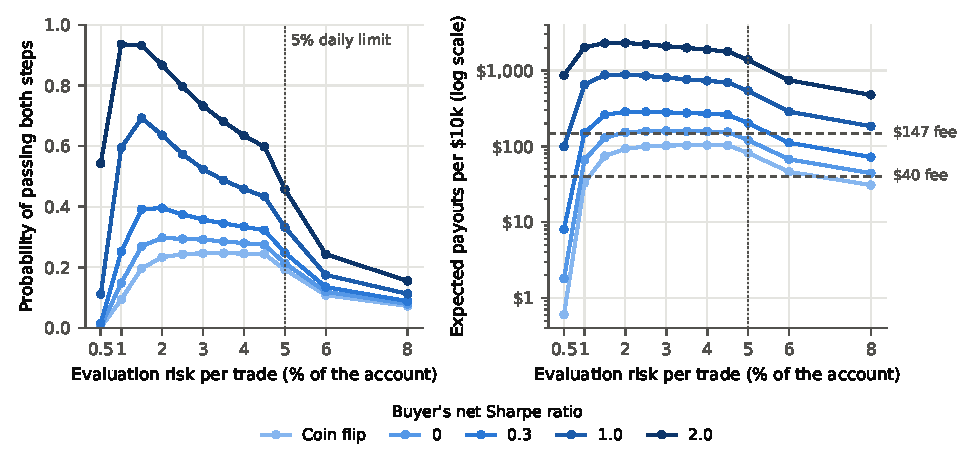
\includegraphics[width=\textwidth]{fig_map.pdf}
\caption{Probability of passing both steps and expected payouts per \$10,000 purchase, by evaluation risk per
trade and the buyer's net Sharpe ratio. Base contract, restricted regime, funded risk 1\%, 36 months.}
\label{fig:map}
\end{figure}

Three features of the sizing grid matter. Value is flat from 3\% to 4.5\% a trade, which is 1.5\% to 2.3\% of
daily volatility and matches the ridge \citet{lim2026} reports near 2\%. At 5\% it falls off a cliff, because a
single stop-out then breaches the daily limit; below 5\% the daily limit never binds on a trade with a stop.
And small sizes are costly: at the 1\% a trade of conventional risk advice the value is \Vconv, and at 0.5\%
almost nothing.

The last point needs a qualification that Section~\ref{sec:horizon} supplies. On a contract with no time limit,
small size mostly costs time. At 1\% a trade, \StillEvalThirtySix{} of no-skill buyers are still in the
evaluation after three years, and the share of value forgone falls from \ForfeitTwelve{} over a 12-month window
to \ForfeitSixty{} over 60 months.

\begin{table}[t]
\centering\small\setlength{\tabcolsep}{5pt}
\begin{threeparttable}
\caption{Selected policy and value by skill, base contract}\label{tab:policy}
\begin{tabular}{lrr rrrr rrrrr}
\toprule
 & & & \multicolumn{4}{c}{Restricted regime ($r_f=1\%$)} & \multicolumn{5}{c}{Standard regime}\\
\cmidrule(lr){4-7}\cmidrule(lr){8-12}
Skill & Sharpe & Hit \% & $r$ \% & P(pass) & P(paid) & $V$ & $r$ \% & $r_f$ \% & P(pass) & P(paid) & $V$\\
\midrule
\tabin{tab_policy}
\bottomrule
\end{tabular}
\begin{tablenotes}\footnotesize
\item $V$ is expected payouts in dollars per \$10,000 purchase within 36 months. Policies are selected on one set
of \Npaths{} paths and reported on another. ``Hit \%'' is the probability of taking the better side of the day.
\end{tablenotes}
\end{threeparttable}
\end{table}

\subsection{Sizing, skill and the horizon}\label{sec:horizon}
Value rises steeply with skill, by about \$40 per 0.1 of Sharpe ratio at the low end (Figure~\ref{fig:skill}a).
A Sharpe ratio of 0.3 is worth \Vskill{}, 2.8 times the coin flip, and the break-even Sharpe ratio at the
\$10,000 list fee is \BEsharpeList, about zero. With skill the best evaluation risk falls to 2\% to 2.5\%.

I had registered three hypotheses on this contract. H1, that the no-skill value lies between the \$40
promotional fee and the \$147 list fee, was supported in the restricted regime and is not robust to the standard
one. H2, that the gain from contract-optimal sizing exceeds the gain from a Sharpe ratio of 0.3, was refuted: the
sizing gain is \SizingGain{} and the skill gain \SkillGain{}, a difference $D$ of \Dval{} (\DvalLo{} to
\DvalHi). H3, that a Sharpe ratio of 0.3 leaves the value below the list fee, was refuted. Both refutations hold
in every robustness row of Table~\ref{tab:hyp}. The skill gain here runs from the coin flip, whose net Sharpe
ratio is \CoinSharpe, to 0.3; measured from a net Sharpe ratio of zero it is \$126, still above sizing.

\begin{figure}[t]
\centering
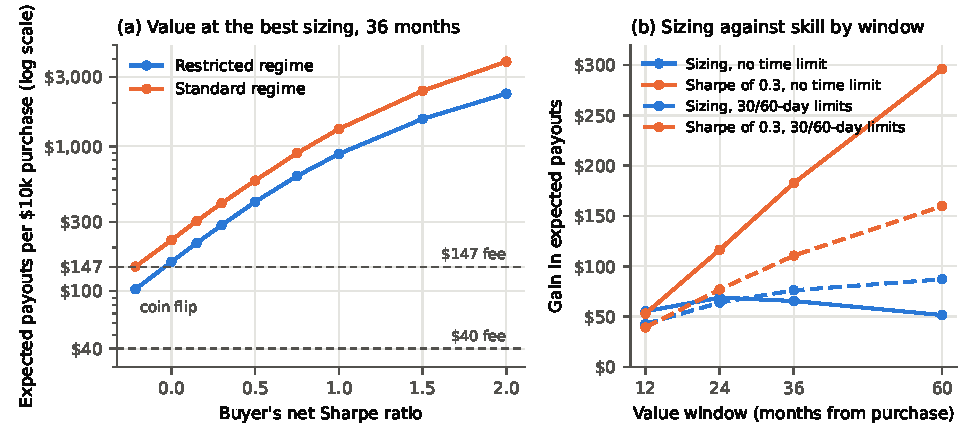
\includegraphics[width=\textwidth]{fig_skill.pdf}
\caption{(a) Expected payouts at each skill level's selected policy, base contract, 36 months. (b) The gain from
sizing (the coin flip moved from 1\% to its best size) and the gain from skill (the coin flip against a Sharpe
ratio of 0.3, each at its best size), by value window, without a time limit and with the classic limits of 30 and
60 trading days. Policies are re-selected in every cell.}
\label{fig:skill}
\end{figure}

This is the opposite of \citet{lim2026}'s reading that ``risk sizing matters at least as much'' as skill. A
second registered run locates the difference (Table~\ref{tab:horizon}, Figure~\ref{fig:skill}b). It crosses the
contract's clock, none or the classic 30 and 60 days, with the value window, 12 to 60 months, and re-selects the
policy in every cell. With the classic clock and a 12-month window, sizing is worth slightly more than skill
($D=$ \DclockTwelve; H4 supported). Without a clock and over 60 months skill is worth far more ($D=$ \DnoneSixty;
H5 supported), and $D$ falls with the window under both clocks (H6 supported). So the length of the window does
most of the work, not the evaluation's time limit: from 24 months on skill leads even with the classic limits.
H7, that $D$ is larger with the clock at every window, was inconclusive at 12 months and supported beyond.

What the clock does is make caution fatal. With the classic limits, a buyer risking 1\% a trade is worth nothing
at any skill level. Without them, a cautious buyer with a Sharpe ratio of 1.0 is worth \CautiousOne{} over
36 months, \CautiousMultiple{} times the best-sized coin flip. Once the buyer re-sizes for it, the clock costs the
coin flip \ClockCostCoin{} of its 36-month value, and \ClockCostOne{} at a Sharpe ratio of 1.0. Measured from a
net Sharpe ratio of zero rather than from the coin flip, sizing is worth more than a step of 0.3 at every window
under the classic clock, which is \citeauthor{lim2026}'s case; it stops holding once the clock is gone and the
buyer stays three years.

\begin{table}[t]
\centering\footnotesize\setlength{\tabcolsep}{4pt}
\begin{threeparttable}
\caption{Value by contract clock and value window}\label{tab:horizon}
\begin{tabular}{llrrrrrrl}
\toprule
 & & \multicolumn{3}{c}{Coin flip} & & \multicolumn{2}{c}{$S=1.0$} & \\
\cmidrule(lr){3-5}\cmidrule(lr){7-8}
Clock & Months & Best size & 1\%/1\% & In eval. & $S=0.3$ & Best & 1\%/1\% & $D$ (95\% interval)\\
\midrule
\tabin{tab_horizon}
\bottomrule
\end{tabular}
\begin{tablenotes}\footnotesize
\item Dollars per \$10,000 purchase, restricted regime, with no cut-off on the evaluation. ``In eval.'' is the
share of coin-flip buyers at 1\%/1\% still in the evaluation at the end of the window. $D$ is the sizing gain minus
the gain from a Sharpe ratio of 0.3.
\end{tablenotes}
\end{threeparttable}
\end{table}

\subsection{What each rule costs}
Table~\ref{tab:rules} removes one rule at a time with the policy held fixed. The largest items are the second
step, trading costs, the firm's 20\% share and the absence of a fee refund. A spread of \CoinCost{} of the risk a
trade takes 28\% of the coin flip's value. The rules \citet{lim2026} lists as omitted from his model are small
here: the Best Day Rule, intraday monitoring, the funded caps and the Max Risk Rule together cost the coin flip
about \$28, taken one at a time, and the daily limit costs nothing. So his caveat that the omissions bias his
values upward is, on this contract, a modest one. The restricted regime is the large one: it lowers the no-skill
value from \VcoinStd{} to \Vcoin. Appendix~\ref{app:more} gives the same table for the standard regime, in which
a skilled buyer is better off without the earliest possible payouts, a point the next subsection measures.

\begin{table}[t]
\centering\small
\begin{threeparttable}
\caption{Change in value when one rule is removed, restricted regime}\label{tab:rules}
\begin{tabular}{lrrr}
\toprule
Rule removed & Coin flip & $S=0.3$ & $S=1.0$\\
\midrule
\tabin{tab_rules}
\bottomrule
\end{tabular}
\begin{tablenotes}\footnotesize
\item Dollars per \$10,000 purchase at each skill level's selected policy, which is held fixed. A buyer who
re-sized would lose less to an added rule and gain more from a removed one; Table~\ref{tab:horizon} re-sizes for
the step maturities.
\end{tablenotes}
\end{threeparttable}
\end{table}

\subsection{The buyer's best policy}\label{sec:best}
Table~\ref{tab:classes} compares four classes of policy on the same real paths: (A) the selected fixed sizes;
(B) those sizes with payout timing free; (C) sizing free with the earliest payout; (D) both free. For the coin
flip the best policy is worth \VbestCoin{} against \Vcoin, a gain of \GainBestCoin{} (H10, a gain above 10\%,
supported), with \PpassBest{} passing and \PpaidBest{} paid. All of the gain comes from sizing.

\begin{table}[t]
\centering\small
\begin{threeparttable}
\caption{Value by class of policy on real paths}\label{tab:classes}
\begin{tabular}{llrrrrr}
\toprule
Regime & Skill & A: fixed & B: A, timing free & C: sizing free & D: both free & D over A\\
\midrule
\tabin{tab_classes}
\bottomrule
\end{tabular}
\begin{tablenotes}\footnotesize
\item Dollars per \$10,000 purchase on the evaluation paths of Table~\ref{tab:policy}. Classes B to D are solved
by backward induction on independent days and then simulated on the real history. In the standard regime 7.5\% of
funded accounts at $S=1.0$ reach the solver's profit cap of \$3,000, so those values are lower bounds.
\end{tablenotes}
\end{threeparttable}
\end{table}

Figure~\ref{fig:policy} shows the policy. Without skill the buyer starts near 4.75\% a trade, shrinks the trade
to just reach the target as it nears, and close to the floor stakes whatever is left. This is the bold play that
\citet{dubins1965} show to be optimal in an unfavourable game, and that \citet{villahermosa2026} invokes. With
skill the policy is cautious: it starts near 2\% to 2.5\%, cuts size as the floor nears and never stakes the
remainder. Average risk in the evaluation falls from \EvalRiskCoin{} without skill to \EvalRiskThree{} at a
Sharpe ratio of 0.3, then edges up to \EvalRiskOne{} at 1.0, because a stronger edge is worth reaching the
funded stage sooner. H11, a monotone fall, is therefore refuted.

\begin{figure}[t]
\centering
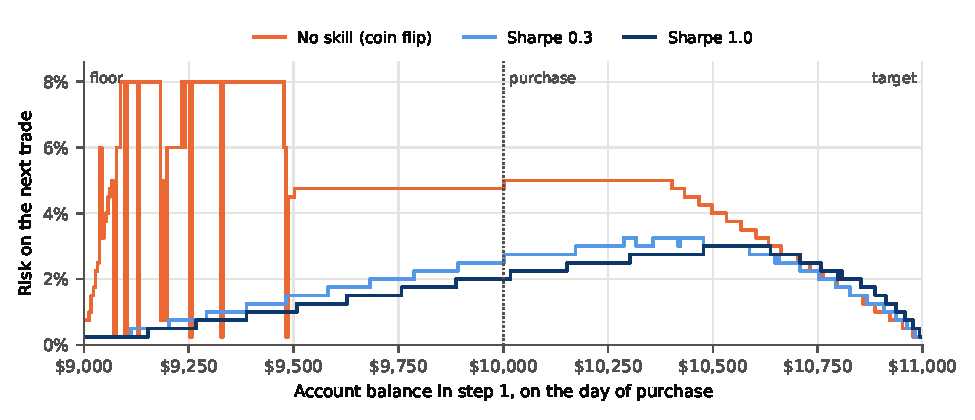
\includegraphics[width=\textwidth]{fig_policy.pdf}
\caption{The best policy's risk on the next trade as a function of the account balance, in step 1 on the day of
purchase, base contract. The irregular sizes close to the floor are near-ties between staking the remainder and
a token trade.}
\label{fig:policy}
\end{figure}

Payout timing matters only with skill (H13 supported). For the coin flip the earliest payout is exactly optimal.
At a Sharpe ratio of 1.0 in the standard regime free timing alone adds \GainTimingOneStd{} and the full policy
\GainBestOneStd: the buyer lets profit build a buffer above the floor before withdrawing. The model of
independent days is adequate: the solver's value exceeds what its policy earns on the real history by a factor
of \ModelRatio{} (H12, within 10\%, supported).

The no-skill policy is the conduct the firm's gambling policy names. On a typical path its largest size is about
\SpanMedian{} times its smallest. The published discretion is therefore aimed at a prize of about a sixth of the
no-skill value; the rest is available at a constant size.

\subsection{The price list}
Table~\ref{tab:menu} and Figure~\ref{fig:menu} price every plan for the same coin-flip buyer. The dispersion is
wide: expected payouts per dollar of list fee run from \PerFeeMin{} on One 6\% to \PerFeeMax{} on Pro 8\%.

\begin{figure}[t]
\centering
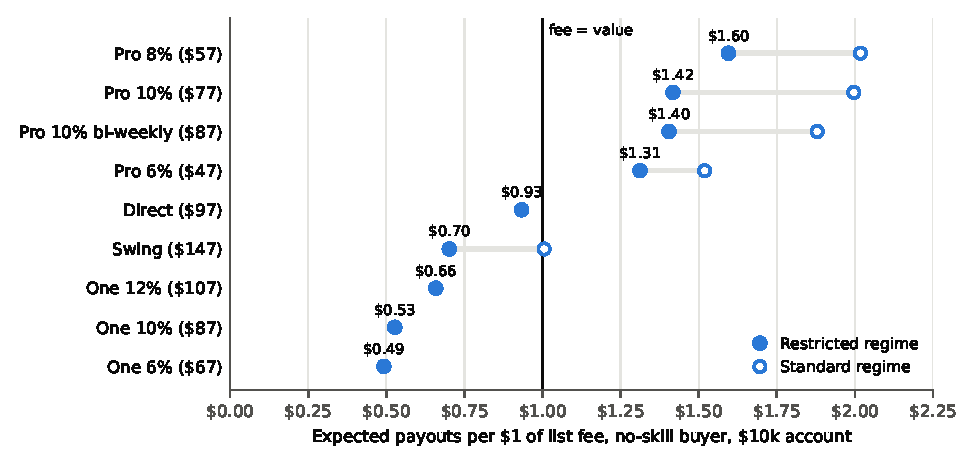
\includegraphics[width=\textwidth]{fig_menu.pdf}
\caption{Expected payouts per dollar of list fee for a no-skill buyer on a \$10,000 account, by plan. List fee in
brackets. Direct has one regime.}
\label{fig:menu}
\end{figure}

\begin{table}[t]
\centering\footnotesize\setlength{\tabcolsep}{3.5pt}
\begin{threeparttable}
\caption{The plan menu at \$10,000 for a no-skill buyer}\label{tab:menu}
\begin{tabular}{lL{3.9cm}rrrrrrrr}
\toprule
Plan & Targets; loss limit & Fee & P(pass) & P(paid) & $V$ & $V$, std. & EV & $V$/fee & $V$, $S=0.3$\\
\midrule
\tabin{tab_menu}
\bottomrule
\end{tabular}
\begin{tablenotes}\footnotesize
\item Dollars per \$10,000 purchase, 36 months, restricted regime unless marked ``std.''. List fees from the
firm's checkout on 13 October 2026. $V$ at $S=0.3$ is at that buyer's own selected policy.
\end{tablenotes}
\end{threeparttable}
\end{table}

Four patterns stand out. Every two-step Pro plan is worth more than its list fee at every account size
(Table~\ref{tab:sizes}); on Pro 10\% the buyer gets back \PerFeeProTen{} per dollar at \$10,000 and
\PerFeeProTenLarge{} at \$100,000. Swing is Pro 10\% at nearly twice the price: the targets and limits are
identical, Pro 10\% is worth \DiffProSwing{} more for this book because its lot cap is looser (H14 supported), and
its value exceeds its \$77 fee by \EVProTen{} (H15 supported). The one-step plans are the poor contracts: One
10\% is worth \DiffOnePro{} less than Pro 10\% (H17 supported), because each payout ratchets the trailing floor up
and the cushion never rebuilds. I had expected Swing to return the least per fee dollar; the One plans do, and
H16 is refuted. Direct is close to fair, \VDirect{} of value against \$97 (H18 supported), with \PpaidDirect{} of
buyers ever paid.

\begin{table}[t]
\centering\small
\begin{threeparttable}
\caption{No-skill expected value at list fees by account size}\label{tab:sizes}
\begin{tabular}{lrrrrrrr}
\toprule
Plan & $V$, \% of account & \$5k & \$10k & \$25k & \$50k & \$100k & \$200k\\
\midrule
\tabin{tab_menu_sizes}
\bottomrule
\end{tabular}
\begin{tablenotes}\footnotesize
\item Dollars per purchase, restricted regime. The rules scale with the account, so $V$ is a constant share of it;
the fee is not.
\end{tablenotes}
\end{threeparttable}
\end{table}

Within each plan the fee per dollar of account falls with size while the value per dollar does not
(Figure~\ref{fig:fee}). On the base contract the list fee is above the no-skill value at \$5,000 and \$10,000 and
below it from \$25,000. A buyer with a Sharpe ratio of 0.3 is above the fee on every plan, by very different
margins: the purchase is worth \VProTenSkill{} on Pro 10\% (fee \$77) and \VOneSixSkill{} on One 6\% (fee \$67).

\begin{figure}[t]
\centering
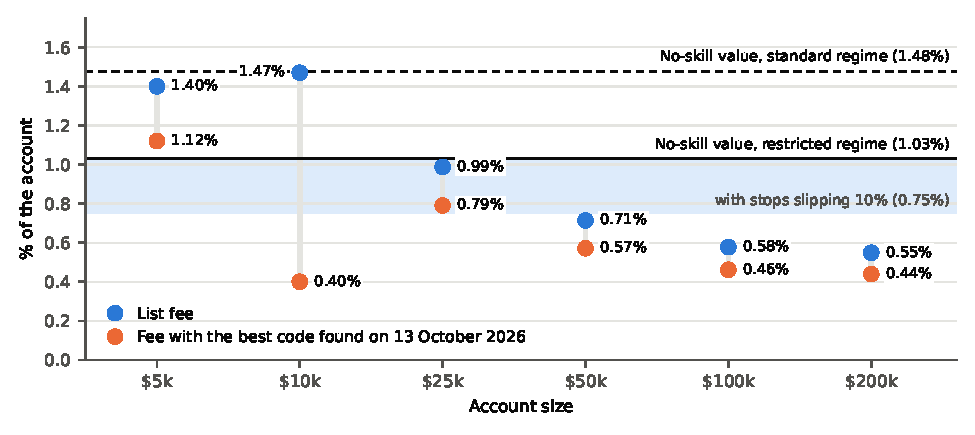
\includegraphics[width=\textwidth]{fig_fee.pdf}
\caption{The base contract's fee as a share of the account, against the no-skill value. The band shows the value
when every stop-out loses 10\% more than the stop distance.}
\label{fig:fee}
\end{figure}

\subsection{Other instruments, stop slippage and robustness}
The figure of about 1\% of the account is specific to the index. I had registered that the no-skill value would
lie between \$75 and \$130 on three other instruments, and it does not (H8 refuted; Table~\ref{tab:books}): it is
\VNas{} on NAS100, \VEur{} on EUR/USD and \VJpy{} on USD/JPY. The differences are trading cost. The value lines
up with the net Sharpe ratio of a random trade, at the same slope as skill in Table~\ref{tab:policy}, so cost
behaves as negative skill; with costs set to zero the four books sit between \$135 and \$165. Skill is worth
more than sizing on every one of them (H9 supported).

\begin{table}[t]
\centering\footnotesize\setlength{\tabcolsep}{4pt}
\begin{threeparttable}
\caption{The base contract on four instruments}\label{tab:books}
\begin{tabular}{lrrrrlrrr}
\toprule
Book & Cost ($R$) & Sharpe & $r$ \% & P(pass) & $V$, coin flip (95\%) & 1\%/1\% & $S=0.3$ & No costs\\
\midrule
\tabin{tab_books}
\bottomrule
\end{tabular}
\begin{tablenotes}\footnotesize
\item The same trade design on each instrument at its own measured spread. ``Cost'' is the mean result of a
random trade in units of risk and ``Sharpe'' its annualised net Sharpe ratio.
\end{tablenotes}
\end{threeparttable}
\end{table}

The simulation's stops never slip: the worst loss in 9,758 simulated trades is exactly the stop distance. An
exploratory stress in which every stop-out loses $1+s$ times that distance lowers the no-skill value on the base
contract to \VslipFive{} at $s=5\%$, \VslipTen{} at 10\% and \VslipTwentyFive{} at 25\%
(Table~\ref{tab:slip}). The size from which the list fee is below the no-skill value moves accordingly. I have no
measurement of slippage on this server; one index point is about 1.2\% of the stop distance.

\begin{table}[t]
\centering\small
\begin{threeparttable}
\caption{Stop slippage (exploratory)}\label{tab:slip}
\begin{tabular}{rrrrl}
\toprule
Slippage $s$ & P(pass) & $V$ & \% of account & List fee below value from\\
\midrule
\tabin{tab_slip}
\bottomrule
\end{tabular}
\begin{tablenotes}\footnotesize
\item Coin flip, base contract, restricted regime, evaluation risk 3.5\%, funded risk 1\%. Not pre-registered.
\end{tablenotes}
\end{threeparttable}
\end{table}

Table~\ref{tab:hyp} gives the registered robustness rows for the base contract: a block bootstrap of days, two
purchase periods, monthly instead of on-demand payouts, a 60-month window and costs at 1.0 and 2.0 times the
measured spread. In those rows the no-skill value ranges from \$92 to \$123, and the refutations of H2 and H3
hold in every row. A discretionary bonus
of 0.25\% of the account on the fourth payout, which the firm publishes and I do not include in $V$, would add
\BonusCoin{} for the coin flip and \BonusOne{} at a Sharpe ratio of 1.0.

\begin{table}[t]
\centering\small
\begin{threeparttable}
\caption{Robustness of H1 to H3 on the base contract}\label{tab:hyp}
\begin{tabular}{L{6.4cm}rrrr}
\toprule
Row & $V$, coin flip & $V$, coin at 1\%/1\% & $V$, $S=0.3$ & $D$\\
\midrule
\tabin{tab_hyp}
\bottomrule
\end{tabular}
\begin{tablenotes}\footnotesize
\item Dollars per \$10,000 purchase. Policies are fixed at the primary selection except in row 1.
\end{tablenotes}
\end{threeparttable}
\end{table}

\subsection{Real paths against the Brownian model}
Passing \citet{lim2026}'s classic contract with the real book in place of his normal increments gives nearly the
same funding probabilities at 2\% daily volatility (0.180 against his 0.184 without skill, and 0.298 against
0.298 at a Sharpe ratio of 1.0; Appendix~\ref{app:more}). At 3\% the real book funds less often, because a
stop-out then exceeds the daily limit. Running normal increments through this paper's contract overstates the
restricted-regime value by about 30\% and shows a rounded peak where the real book shows a plateau and a cliff.
The differences between his contract values and mine therefore come mostly from the rules, in particular the
absent time limit, on-demand payouts and three years of funded trading, and not from the paths.

\section{Is the skill there?}\label{sec:skill}
The contract pays for skill. Whether a buyer has any is a separate question, and the one this paper can speak to
only for one kind of buyer: a researcher who tests published effects carefully at retail costs.

\paragraph{Twenty-four tests.} Before this study I ran a programme of 24 pre-registered tests of published
trading effects on currency, index, bond and commodity contracts at the same broker's measured spreads and swaps,
with a discovery sample, a validation sample, one-time hold-outs, random-timing twins and a Benjamini--Hochberg
correction across the family \citep{benjamini1995}. The ideas came from work on currency fixings
\citep{krohn2024}, month-end hedging flows \citep{melvin2015}, monetary policy announcements
\citep{mueller2017,lee2025}, futures positioning \citep{tornell2012}, value, momentum and trend
\citep{asness2013,moskowitz2012}, cryptocurrency momentum \citep{liu2021}, macroeconomic announcements
\citep{andersen2003}, earnings drift \citep{bernard1989}, statistical arbitrage \citep{avellaneda2010,gatev2006},
news tone \citep{tetlock2007}, Treasury auctions \citep{lou2013} and the turn of the month
\citep{lakonishok1988}, together with machine-learning and positioning signals. None was confirmed. Several
effects were present before costs and absent after them: slow strategies lost to swaps and fast ones to spreads.

\begin{figure}[t]
\centering
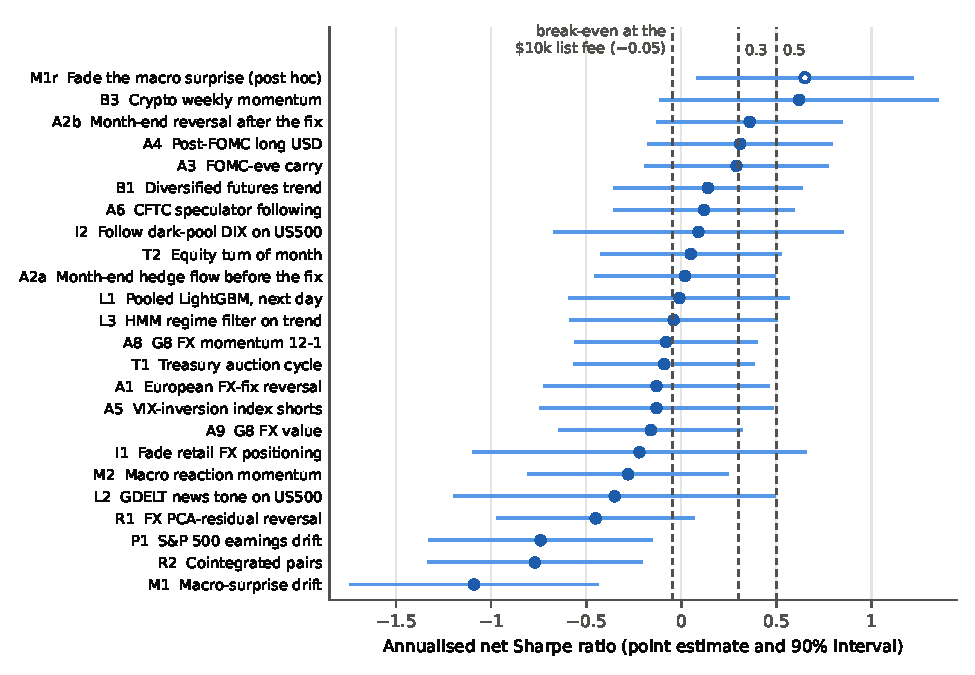
\includegraphics[width=0.92\textwidth]{fig_tests.pdf}
\caption{Annualised net Sharpe ratio of each of the 24 tests on the sample that decided it, with a 90\% interval
\citep{lo2002}. The hollow marker is a strategy whose sign was chosen after its parent test.}
\label{fig:tests}
\end{figure}

\paragraph{What the tests can and cannot exclude.} Figure~\ref{fig:tests} reports each test under a rule fixed
in the plan, following the reporting convention of \citet{darmanin2026}: a test refutes a Sharpe ratio of $S^*$
if the upper end of its one-sided 95\% interval lies below $S^*$. At $S^*=0.5$, \RefutedFive{} of the 24 are
refuted. At 0.3, only \RefutedThree{} are. The median test could have detected a Sharpe ratio of \MdeMedian{} with
80\% power. ``No edge was found'' is supported; ``no edge exists'' is not.

This is not a weakness peculiar to the programme. The contract's break-even Sharpe ratio is about zero, and a
ratio of 0.3 doubles its value, so the purchase turns on a difference of a few tenths. Telling a Sharpe ratio of
0.3 from zero with 80\% power at the 5\% level takes about 69 years of daily data. No retail track record and few
backtests resolve the range that decides the purchase. The evaluation does not resolve it either: \Ppass{} of
no-skill buyers pass, against 37.5\% at a Sharpe ratio of 0.3, so a pass multiplies the odds of that much skill
by about 1.5.

\paragraph{Real strategies through the contract.} The skilled buyer of Section~\ref{sec:results} is idealised.
Table~\ref{tab:real} runs the programme's surviving strategies through the base contract as they actually trade:
three forward-test candidates and two ensembles of them, each converted to a daily series at one unit of risk per
trade. None is a confirmed edge, and two were chosen after their parent tests were seen, which flatters them on
early purchases. Sizes are selected on purchases from 2005 to 2014 and held for purchases from 2017 to 2021.

\begin{table}[t]
\centering\footnotesize\setlength{\tabcolsep}{4pt}
\begin{threeparttable}
\caption{The programme's surviving strategies through the base contract}\label{tab:real}
\begin{tabular}{L{4.2cm}lrrrrlr}
\toprule
Book & Purchases & Sharpe & P(pass) & Months & P(paid) & $V$ (95\% interval) & Idealised\\
\midrule
\tabin{tab_real}
\bottomrule
\end{tabular}
\begin{tablenotes}\footnotesize
\item Dollars per \$10,000 purchase, restricted regime. ``Idealised'' is the value of the Section~\ref{sec:method}
buyer at the same net Sharpe ratio on the same purchase days. Intervals are from a stationary bootstrap of the
purchase days \citep{politis1994}, because neighbouring purchases share most of their path. ``Months'' is the
median time to pass.
\end{tablenotes}
\end{threeparttable}
\end{table}

Every book is worth less than an idealised buyer with the same Sharpe ratio (H19 supported). The ensemble that
was tested on untouched data has a Sharpe ratio of \SharpeRthreeLate{} on late purchases and is worth
\VRthreeLate, against \IdealRthreeLate. Two mechanisms do this. An event-driven edge trades too rarely to reach
the targets: the month-end book trades on about twelve days a year and passes 1\% of the time at any size. And
once funded, the restricted regime caps the risk of all open positions together at 1\%, so a book with twelve
trades open risks 0.08\% on each. The one book that trades daily is worth \VAoneEarly{} on the years it was
chosen on and \VAoneLate{} afterwards, with an interval from \VAoneLateLo{} to \VAoneLateHi. Whether it beats the
no-skill buyer's \CoinLate{} on the same purchase days is not settled (H20 inconclusive), and nor is whether
every book has decayed (H21 inconclusive): five overlapping years hold few independent three-year windows.

The \Vskill{} that the contract pays for a Sharpe ratio of 0.3 is thus the price of an edge that trades one
position every day. The programme produced nothing of that kind.

\section{The seller's side}\label{sec:seller}
I observe nothing of the firm's books, so this section draws implications and no more.

\paragraph{Who pays.} The same contract returns very different amounts to different buyers.
On the base contract at its \$147 list fee, expected payouts per dollar of fee are \$0.22 for a no-skill buyer at
conventional 1\% sizing, \PerFeeSwing{} at contract-optimal sizing and \$1.94 at a Sharpe ratio of 0.3; on Pro
10\% the middle figure is \PerFeeProTen. A seller whose buyers were all disciplined would lose money on most of
its menu at list prices. It does not need to exclude them if they are few. \citet{lim2026} reaches the same
conclusion from an assumed population, attributing the margin to cost drag and to buyers sizing away from the
ridge, and \citet{villahermosa2026} from the pass rate at which his seller breaks even. The only public figure I
could read at its source is a trade-press report of a technology vendor's data, in which 7\% of 300,000 accounts
across ten firms achieved a payout and payouts averaged 4\% of the account \citep{financemagnates2025}. Taken at
face value that is about 0.3\% of the account per purchase, against \VcoinPct{} for the disciplined no-skill buyer
here and 0.33\% at 1\% sizing. The firms, rules and dates differ, the figure is not audited, and I do not rest
anything on it. It is consistent with a customer base that does about as well as a no-skill buyer following
conventional risk advice.

\paragraph{What the price list suggests.} The menu's pricing is hard to explain by the cost of the claims. Fees
fall with account size while the value of the claim per dollar does not. Two plans with identical targets and
limits differ in price by a factor of two. And the plans that are simplest to describe, one step or none, carry
the least value per fee dollar. These patterns fit prices set by what buyers will pay for salient features,
such as a single step, weekend holding or a large notional balance, more than by the claims' actuarial value.
That is a conjecture; the data that would test it are the firm's.

\paragraph{Discretion.} If the rules do not protect the seller against a disciplined buyer, something else must.
The published restriction regime removes 30\% of the no-skill value on the base contract. The gambling policy is
aimed at the state-dependent sizing worth a further sixth. Beyond those, the terms reserve review of every pass
and every payout. At the \$40 promotional fee available on the base contract's \$10,000 account, the no-skill
buyer's expected value is zero if \DenialPromo{} of payouts are refused. I cannot observe how often any of this is
used. The point for disclosure policy is that an average pass rate or payout ratio, as \citet{lim2026} proposes
firms should publish, would describe the firm's customers and its discretion as much as its contract. Both are
worth knowing; they are not the same thing as the odds the rules imply.

\section{Limitations}\label{sec:limits}
\emph{One firm, one date.} The rules and fees are one firm's on 13 October 2026. They change; the rule sources are
dated and hashed so that the contract priced here can be identified.

\emph{The firm pays.} Every value assumes each valid request is paid. Discretionary refusal, the gambling
policy, the review on passing and the ``same level of risk'' clause are not modelled.

\emph{One trade design.} The no-skill book is one intraday trade a day with a stop. Other books would differ;
the four instruments of Table~\ref{tab:books} show by how much cost alone moves the value.

\emph{Execution.} Costs are one broker's spreads measured in 2026 and applied to 2005 to 2024 in proportion to
price. Stops fill at the stop price in the base case. The five-minute news restriction on the Pro, One and Direct
plans is not modelled; the trade avoids scheduled releases by design, but a stop triggered inside a window would
be a close inside it.

\emph{Skill is idealised.} Section~\ref{sec:skill} shows how far real strategies fall short of it.

\emph{A machine with three years.} The buyer never deviates, trades every day for up to 36 months and takes each
payout mechanically. About 75\% of no-skill purchases fail and 85\% are never paid, so the expected value is the
mean of a skewed distribution and a single buyer should expect to lose the fee.

\emph{Pre-registration.} The plans were committed to a private research repository before the runs they describe.
The history of the plan and of every commit touching the analysis is in the reproduction package's
\texttt{provenance/} folder, and the full repository is available to editors and referees on request. Git dates can
be set by the author, so this is a record rather than proof; later plans will be registered with a third party
before they are run. The 24 tests were run in adaptive batches and their family was fixed as it grew.

\emph{Unrefereed neighbours.} The three papers closest to this one are working papers. I reproduced the one whose
numbers I use and cite the others as reported.

\section{Conclusion}\label{sec:conclusion}
On its written rules, the contract examined here is close to a fair bet for a disciplined buyer with no skill
and a cheap claim for one with a little. Its base plan returns about 1\% of the account in expected payouts
against a fee of 0.55\% to 1.47\%; the firm's standard two-step plans return more than their list fee at every
size; its one-step plans return about half of theirs. The value depends on the instrument's trading cost, on
stops filling, and on the firm paying.

The rules are not what defeats buyers. The time limit is gone, the daily limit does not bind a stopped trade and
the consistency rule costs a tenth. What stands between a buyer and the contract's value is sizing that suits
ordinary risk advice and not this contract, the absence of an edge that 24 registered tests did not find and no
track record could verify, and the seller's discretion over the conduct that extracts value without skill.

For buyers, the practical reading is narrow: passing an evaluation is weak evidence of skill, and the expected
value of a single purchase is the mean of a distribution in which most purchases return nothing. For regulators,
disclosure of realised pass and payout rates would be informative about a firm's customers and conduct, and
should be read alongside the odds its rules imply, which this paper shows can be computed from public documents.
For research, the method extends to any firm that publishes its rules, and the solved contract offers a test bed
with a known optimum.

\appendix
\section{Rule sources}\label{app:rules}
All pages were fetched directly on 13 October 2026 from \url{https://help.alphacapitalgroup.uk} and
\url{https://alphacapitalgroup.uk/terms-and-conditions}. The repository records each page's address, date and
SHA-256 hash and the script that checks every quoted phrase against the raw page.

\begin{longtable}{L{3.0cm}L{8.2cm}L{3.6cm}}
\toprule
Rule & As published & Source article (page date)\\
\midrule
\endhead
Targets & ``Phase 1 profit target: 10\%'', ``Phase 2 profit target: 5\%'' & Alpha Swing (24 Jul 2026)\\
Overall loss & ``Max Drawdown (static): 10\%''; ``If the balance or equity drops below \$90,000, the account is breached'' & Alpha Swing; Maximum total loss (24 Jul 2026)\\
Daily loss & ``Max Daily Drawdown (balance-based): 5\%''; ``breaches are always applied based on open trades (unrealised losses)'' & Daily risk limits (24 Jul 2026)\\
Minimum days & ``Minimum trading days (for each phase): 3''; a trading day is ``a day on which you open and close a trade on the same day'' & Alpha Swing; Minimum trading days (6 Jul 2026)\\
Time limit & ``There are no time limits applicable to the Evaluations'' & Terms, clause 8.2.1\\
Evaluation size & ``There is no maximum virtual position size exposure during the evaluation stage'' & Terms, Schedule 2, 3.4(a)\\
Inactivity & ``All accounts, at all stages'' are subject to a 30-day inactivity limit & Inactivity (6 Jul 2026)\\
Refund & ``All our evaluation plans are non-refundable'' & Refund of evaluation fees (6 Jul 2026)\\
Commission & ``Indices are commission-free across both account types'' & Commission fees (6 Jul 2026)\\
Lot cap & Swing: \$10k = max 2.5 lots; ``the total combined lots/position size allowed at any one time'' & Lot size limit (21 Jul 2026)\\
Max Risk Rule & ``applies to Qualified Accounts only''; 3\% up to \$25,000 and 2\% from \$50,000, on ``floating/unrealised losses'' & Max Risk Rule (25 Aug 2026)\\
Payout & ``a minimum of 2\% of gross profits on the account balance''; ``no single trading day should contribute more than a set percentage of the total generated profits'' (40\%) & On-demand performance fee (22 Jul 2026)\\
Processing & ``processed and paid within 2 business days''; ``You can resume trading once your account balance has been reset'' & How do I get paid (7 Jul 2026)\\
Split & ``an 80\% share of the profits'' & What Qualified Analysts earn (21 Jul 2026)\\
Bonus & ``on the fourth performance fee request, a discretionary bonus of 0.25\% of the initial account size is applied'' & Performance fee bonus (7 Jul 2026)\\
Restricted group & ``a temporary group into which Qualified Analyst accounts may be moved''; ``the maximum allowable risk for any single position is 1\% of your initial balance''; Swing lots halved, index leverage 1:5 & Focused Trader Group (7 Sep 2026)\\
Gambling policy & ``A significant change in lot size compared to the overall average on the account''; ``all or nothing''; ``the removal of profits'' & Policy against gambling (6 Jul 2026)\\
Same risk & ``A Qualified Analyst is required to maintain the same level of risk on a Qualified Analyst Account'' & Terms, Schedule 2, 3.2\\
Review & ``All passed evaluations are subject to review, and traders found guilty of policy ignorance or abuse will not advance to the Qualified phase'' & Prohibited trading strategies\\
Allocation & ``a maximum allocation of \$400,000 per household''; ``a \$300,000 limit per strategy'' & How many accounts (6 Jul 2026)\\
Scaling & At a 10\% gain the trader ``can request scaling''; not available in the restricted group & Scaling plan (24 Jul 2026)\\
\bottomrule
\end{longtable}

\noindent Not modelled: the fourth-payout bonus (priced separately in Section~\ref{sec:results}), the scaling plan
(which cannot help a buyer who takes each payout at 2\% and is closed to the restricted group), the allocation
caps, the news rule and the discretionary clauses.

\section{Hypotheses and verdicts}\label{app:verdicts}
\begin{table}[h]
\centering\footnotesize
\begin{threeparttable}
\caption{All registered hypotheses}\label{tab:verdicts}
\begin{tabular}{lL{6.1cm}L{4.9cm}l}
\toprule
 & Hypothesis & Estimate (95\% interval) & Verdict\\
\midrule
\tabin{tab_verdicts}
\bottomrule
\end{tabular}
\begin{tablenotes}\footnotesize
\item $D$ is the gain from contract-optimal sizing minus the gain from a Sharpe ratio of 0.3. A hypothesis is
supported if the interval excludes its boundary in the stated direction, refuted if it excludes it in the other,
and inconclusive otherwise. H1 to H3 were fixed in the original plan; H4 to H9, H10 to H13, H14 to H18 and H19
to H21 in four dated amendments, each committed before its run.
\end{tablenotes}
\end{threeparttable}
\end{table}

\section{Further tables}\label{app:more}
\begin{table}[h]
\centering\small
\begin{threeparttable}
\caption{The coin flip along the sizing grid, base contract, restricted regime}\label{tab:coin}
\begin{tabular}{rrrrrrrrrr}
\toprule
$r$ \% & Daily vol.\ \% & P(step 1) & P(pass) & Months & Static & Daily & In eval. & P(paid) & $V$\\
\midrule
\tabin{tab_coin}
\bottomrule
\end{tabular}
\begin{tablenotes}\footnotesize
\item ``Static'' and ``Daily'' are the shares of purchases that breach each limit in the evaluation; ``In eval.''
the share still in it after 504 trading days. Funded risk 1\%.
\end{tablenotes}
\end{threeparttable}
\end{table}

\begin{table}[h]
\centering\small
\begin{threeparttable}
\caption{Change in value when one rule is removed, standard regime}\label{tab:rulesstd}
\begin{tabular}{lrrr}
\toprule
Rule removed & Coin flip & $S=0.3$ & $S=1.0$\\
\midrule
\tabin{tab_rules_std}
\bottomrule
\end{tabular}
\end{threeparttable}
\end{table}

\begin{table}[h]
\centering\small
\begin{threeparttable}
\caption{Funding probabilities on \citet{lim2026}'s classic contract}\label{tab:lim}
\begin{tabular}{rrrrrrr}
\toprule
 & & \multicolumn{2}{c}{Normal increments} & \multicolumn{3}{c}{Real book}\\
\cmidrule(lr){3-4}\cmidrule(lr){5-7}
Sharpe & Vol.\ \% & Lim & This paper & $r$ \% & At the close & Intraday\\
\midrule
\tabin{tab_lim}
\bottomrule
\end{tabular}
\begin{tablenotes}\footnotesize
\item Probability of passing both steps of his Table~1 contract. ``This paper'' is my simulator with his contract
and normal increments. The real book is sized to the same daily volatility.
\end{tablenotes}
\end{threeparttable}
\end{table}

\begin{table}[h]
\centering\small
\begin{threeparttable}
\caption{The base contract's fee and the no-skill value by account size}\label{tab:fee}
\begin{tabular}{lrrrrrrr}
\toprule
Account & List fee & \% & EV at list & Coded fee & \% & EV with code & Refusal rate\\
\midrule
\tabin{tab_fee}
\bottomrule
\end{tabular}
\begin{tablenotes}\footnotesize
\item Coin flip, restricted regime. ``Coded fee'' is the lowest fee obtained with a discount code at checkout on
13 October 2026. ``Refusal rate'' is the share of payouts that would have to be refused for the coded expected
value to be zero.
\end{tablenotes}
\end{threeparttable}
\end{table}

{\scriptsize\setlength{\tabcolsep}{3.5pt}
\begin{longtable}{lL{4.3cm}rrlrlll}
\caption{The 24 tests: claim exclusion}\label{tab:tests}\\
\toprule
Test & Idea & Years & Sharpe & 90\% interval & MDE & At $S^*$ & At 0.3 & At 0.5\\
\midrule
\endhead
\tabin{tab_tests}
\bottomrule
\end{longtable}
\noindent $S^*$ is the break-even Sharpe ratio at the base contract's \$10,000 list fee (\BEsharpeList). MDE is the
Sharpe ratio detectable with 80\% power at the one-sided 5\% level. Intervals follow \citet{lo2002}.}

\begin{thebibliography}{99}
\bibitem[Andersen et~al.(2003)]{andersen2003} Andersen, T. G., Bollerslev, T., Diebold, F. X., \& Vega, C. (2003).
Micro effects of macro announcements: Real-time price discovery in foreign exchange. \emph{American Economic
Review}, 93(1), 38--62.
\bibitem[Asness et~al.(2013)]{asness2013} Asness, C. S., Moskowitz, T. J., \& Pedersen, L. H. (2013). Value and
momentum everywhere. \emph{Journal of Finance}, 68(3), 929--985.
\bibitem[Avellaneda and Lee(2010)]{avellaneda2010} Avellaneda, M., \& Lee, J.-H. (2010). Statistical arbitrage in
the US equities market. \emph{Quantitative Finance}, 10(7), 761--782.
\bibitem[Benjamini and Hochberg(1995)]{benjamini1995} Benjamini, Y., \& Hochberg, Y. (1995). Controlling the false
discovery rate: A practical and powerful approach to multiple testing. \emph{Journal of the Royal Statistical
Society: Series B}, 57(1), 289--300.
\bibitem[Bernard and Thomas(1989)]{bernard1989} Bernard, V. L., \& Thomas, J. K. (1989). Post-earnings-announcement
drift: Delayed price response or risk premium? \emph{Journal of Accounting Research}, 27 (Supplement), 1--36.
\bibitem[Darmanin(2026)]{darmanin2026} Darmanin, A. (2026). Retail trader's ruin: An anatomy of popular signal
failure. arXiv:2607.20093 (working paper, not peer reviewed).
\bibitem[Dubins and Savage(1965)]{dubins1965} Dubins, L. E., \& Savage, L. J. (1965). \emph{How to Gamble If You
Must: Inequalities for Stochastic Processes}. McGraw-Hill.
\bibitem[Finance Magnates(2025)]{financemagnates2025} Finance Magnates (2025). Only 1 in 20 traders pass prop firm
challenges, reports The Funded Trader. 18 March.
\url{https://www.financemagnates.com/forex/only-1-in-20-traders-pass-prop-firm-challenges-reports-the-funded-trader/}
(accessed 13 October 2026).
\bibitem[Gatev et~al.(2006)]{gatev2006} Gatev, E., Goetzmann, W. N., \& Rouwenhorst, K. G. (2006). Pairs trading:
Performance of a relative-value arbitrage rule. \emph{Review of Financial Studies}, 19(3), 797--827.
\bibitem[Krohn et~al.(2024)]{krohn2024} Krohn, I., Mueller, P., \& Whelan, P. (2024). Foreign exchange fixings and
returns around the clock. \emph{Journal of Finance}, 79(1), 541--578.
\bibitem[Lakonishok and Smidt(1988)]{lakonishok1988} Lakonishok, J., \& Smidt, S. (1988). Are seasonal anomalies
real? A ninety-year perspective. \emph{Review of Financial Studies}, 1(4), 403--425.
\bibitem[Lee and Wang(2025)]{lee2025} Lee, S. S., \& Wang, M. (2025). Jumps and post-FOMC announcement returns in
currency markets. \emph{Review of Asset Pricing Studies}, 15(3--4), 247--287.
\bibitem[Lim(2026)]{lim2026} Lim, B. C. (2026). The price of a funded account: An actuarial analysis of
proprietary trading firm challenges. SSRN working paper 7178078 (not peer reviewed).
\bibitem[Liu and Tsyvinski(2021)]{liu2021} Liu, Y., \& Tsyvinski, A. (2021). Risks and returns of cryptocurrency.
\emph{Review of Financial Studies}, 34(6), 2689--2727.
\bibitem[Lo(2002)]{lo2002} Lo, A. W. (2002). The statistics of Sharpe ratios. \emph{Financial Analysts Journal},
58(4), 36--52.
\bibitem[Lou et~al.(2013)]{lou2013} Lou, D., Yan, H., \& Zhang, J. (2013). Anticipated and repeated shocks in
liquid markets. \emph{Review of Financial Studies}, 26(8), 1891--1912.
\bibitem[Melvin and Prins(2015)]{melvin2015} Melvin, M., \& Prins, J. (2015). Equity hedging and exchange rates at
the London 4 p.m.\ fix. \emph{Journal of Financial Markets}, 22, 50--72.
\bibitem[Moskowitz et~al.(2012)]{moskowitz2012} Moskowitz, T. J., Ooi, Y. H., \& Pedersen, L. H. (2012). Time series
momentum. \emph{Journal of Financial Economics}, 104(2), 228--250.
\bibitem[Mueller et~al.(2017)]{mueller2017} Mueller, P., Tahbaz-Salehi, A., \& Vedolin, A. (2017). Exchange rates
and monetary policy uncertainty. \emph{Journal of Finance}, 72(3), 1213--1252.
\bibitem[Politis and Romano(1994)]{politis1994} Politis, D. N., \& Romano, J. P. (1994). The stationary bootstrap.
\emph{Journal of the American Statistical Association}, 89(428), 1303--1313.
\bibitem[Tetlock(2007)]{tetlock2007} Tetlock, P. C. (2007). Giving content to investor sentiment: The role of media
in the stock market. \emph{Journal of Finance}, 62(3), 1139--1168.
\bibitem[Tornell and Yuan(2012)]{tornell2012} Tornell, A., \& Yuan, C. (2012). Speculation and hedging in the
currency futures markets: Are they informative to the spot exchange rates. \emph{Journal of Futures Markets},
32(2), 122--151.
\bibitem[Villahermosa(2026)]{villahermosa2026} Villahermosa, R. (2026). Prop-firm challenges: A barrier model of
pass rates and expected value. SSRN working paper 7445798 (not peer reviewed).
\end{thebibliography}

\end{document}
